\chapter{Μεθοδολογία και Υλοποίηση}
\label{chapter:implementations}

Στόχος της παρούσας εργασίας είναι να παρέχει στον χρήστη μια απλοποιημένη διαδικασία ώστε να παράγεται κώδικας βασισμένος στις συσκευές στις οποίες διαθέτει, ο οποίος θα εκτελεστεί μετέπειτα στο λειτουργικό RIOT. Κατά αυτόν τον τρόπο, ο χρήστης μπορεί να κατασκευάσει μια εφαρμογή με τις IoT συσκευές που διαθέτει, η οποία θα εκτελεί κάποιες αρκετά βασικές λειτουργίες, χωρίς να χρειάζεται να αναλωθεί στο να βρει τον τρόπο με τον οποίο υποστηρίζονται οι συσκευές αυτές από το RIOT.

Για να επιτευχθεί αυτός ο στόχος, αρχικά σχεδιάστηκαν κάποια μετα-μοντέλα που περιέχουν χαρακτηριστικά συσκευών και των συνδέσεων μεταξύ τους. Μέσω ενός εργαλείου κειμένου, ο χρήστης πρέπει να ορίσει τα χαρακτηριστικά που επιθυμεί να έχει το δικό του σύστημα (σύμφωνα πάντα με τους κανόνες των μετα-μοντέλων). Αφού γίνει αυτό, πραγματοποιούνται μετασχηματισμοί M2M από μοντέλα κειμένου σε διαγράμματα, μέσω των οποίων ο χρήστης μπορεί πιο εύκολα να αντιληφθεί πως ακριβώς θα πρέπει να είναι η συνδεσμολογία μεταξύ των συσκευών του. Τέλος, από τα μοντέλα γίνεται και πάλι μετασχηματισμός (αυτή τη φορά M2T) σε αρχεία κώδικα, τα οποία θα είναι έτοιμα ώστε να γίνει η εγγραφή τους στις συσκευές και άρα να εκτελεστούν.

Όλα όσα υλοποιήθηκαν, περιγράφονται αναλυτικά σε αυτήν την ενότητα.

\section{Ορισμός μετα-μοντέλου Συσκευής}
\label{sec:metamodel_device}

Το μετα-μοντέλο αυτό περιέχει χαρακτηριστικά που μπορεί να έχει μια συσκευή (μικροελεγκτής ή περιφερειακό) και μας χρησιμεύουν στη διαδικασία παραγωγής κώδικα. Στο \autoref{fig:metamodel_device} μπορούμε να δούμε μία απεικόνισή του.

\begin{figure}[!ht]
	\centering
	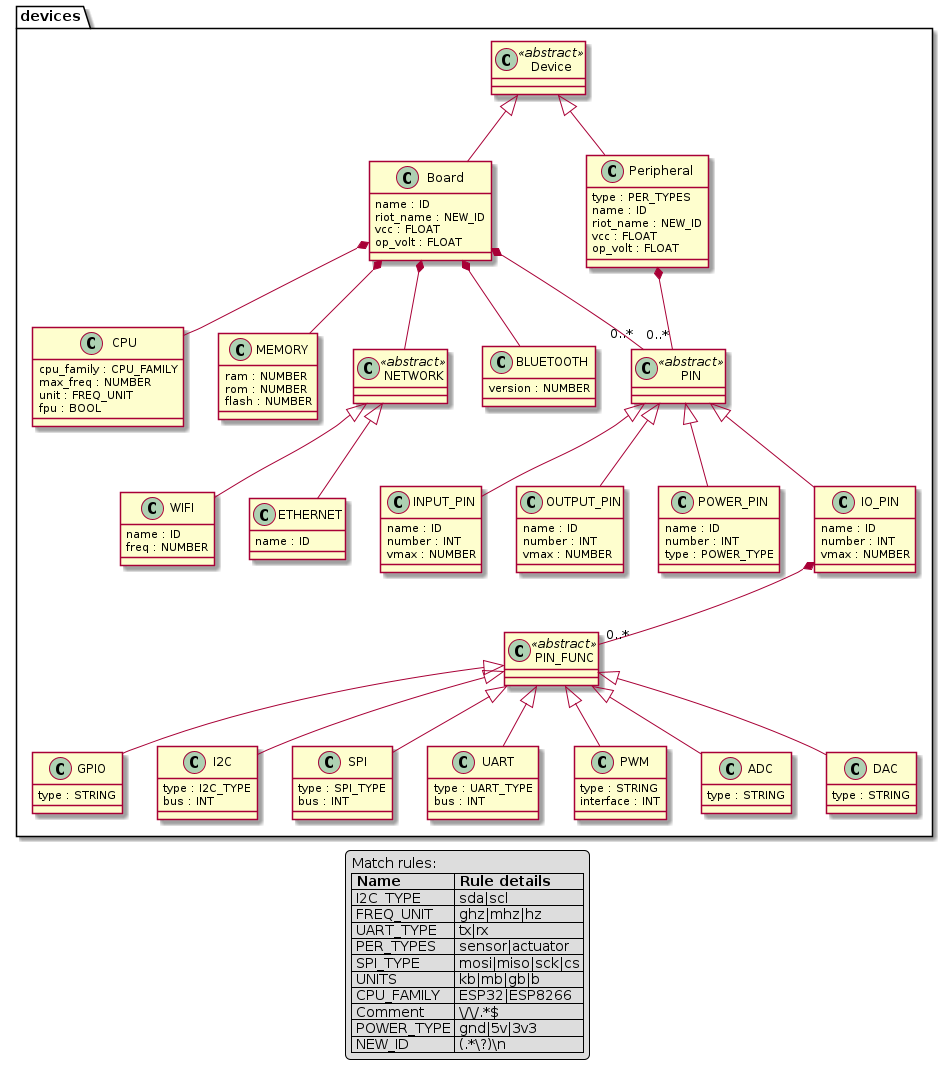
\includegraphics[height=0.8\textheight]{./images/chapter5/metamodel_device.png}
	\caption{Μετα-μοντέλο συσκευής}
	\label{fig:metamodel_device}
\end{figure}

\subsection{Device}
\label{subsec:device}

\subsubsection*{Σύνοψη}

\noindent Το στοιχείο αυτό είνια η abstract κλάση για το αν μια συσκευή είναι μικροελεγκτής ή περιφερειακό.

\subsubsection*{Ιδιότητες και Συσχετίσεις}

\noindent Δεν περιλαμβάνει περαιτέρω ιδιότητες και συσχετίσεις.

\subsubsection*{Περιορισμοί}

\noindent Δεν υπάρχουν περιορισμοί.

\subsection{Board}
\label{subsec:board}

\subsubsection*{Σύνοψη}

\noindent Το στοιχείο αυτό αναπαριστά τις υπολογιστικές συσκευές (μικροελεγκτές).

\subsubsection*{Ιδιότητες και Συσχετίσεις}

\begin{table}[H]
	\begin{center}
		\caption{Ιδιότητες του \textit{Board}.}
		\label{tab:board1}
		\begin{tabular}{ | c | c | c| m{5.5cm} | }
			\hline
			\rowcolor{Gray}
			Όνομα & Τύπος & Πολλαπλότητα & Περιγραφή \\
			\hline
			name & ID & 1..1 &  Το όνομα της συσκευής \\
			\hline
			riot\_name & NEW\_ID & 1..1 &  Το όνομα της συσκευής όπως αναγνωρίζεται από το RIOT \\
			\hline
			vcc & FLOAT & 1..1 & Η τάση τροφοδοσίας της συσκευής \\
			\hline
			op\_volt & FLOAT & 1..1 &  Η τάση λειτουργίας της συσκευής \\
			\hline
		\end{tabular}
	\end{center}
\end{table}

\begin{table}[H]
	\begin{center}
		\caption{Συσχετίσεις του \textit{Board}.}
		\label{tab:board2}
		\begin{tabular}{ | c | c | c| m{5.5cm} | }
			\hline
			\rowcolor{Gray}
			Όνομα & Τύπος & Πολλαπλότητα & Περιγραφή \\
			\hline
			Device & SuperType-Επέκταση & - &  Το στοιχείο Board επεκτείνει το στοιχείο Device \\
			\hline
			CPU & Composition-Σύνθεση & 1..1 &  Η κεντρική μονάδα επεξεργασίας της συσκευής \\
			\hline
			MEMORY & Composition-Σύνθεση & 1..1 &  Η μνήμη της συσκευής \\
			\hline
			NETWORK & Composition-Σύνθεση & 0..1 &  Πρωτόκολλα δικτύου που υποστηρίζει η συσκευή \\
			\hline
			PIN & Composition-Σύνθεση & 0..* &  Οι ακροδέκτες της συσκευής \\
			\hline
			BLUETOOTH & Composition-Σύνθεση & 0..1 &  Υποστήριξη bluetooth \\
			\hline
		\end{tabular}
	\end{center}
\end{table}

\subsubsection*{Περιορισμοί}

\noindent Το riot\_name μπορεί να πάρει τιμές σαν ID, με επιπλέον επιλογή να περιλαμβάνει και παύλες. Αυτό γίνεται μέσω του NEW\_ID που είναι μια \textit{κανονική έκφραση}.

\subsection{Peripheral}
\label{subsec:peripheral}

\subsubsection*{Σύνοψη}

\noindent Το στοιχείο αυτό αναπαριστά τα περιφερειακά.

\subsubsection*{Ιδιότητες και Συσχετίσεις}

\begin{table}[H]
	\begin{center}
		\caption{Ιδιότητες του \textit{Peripheral}.}
		\label{tab:peripheral1}
		\begin{tabular}{ | c | c | c| m{5.5cm} | }
			\hline
			\rowcolor{Gray}
			Όνομα & Τύπος & Πολλαπλότητα & Περιγραφή \\
			\hline
			type & PER\_TYPES (Enum) & 1..1 &  Ο τύπος του περιφερειακού \\
			\hline
			name & ID & 1..1 &  Το όνομα της συσκευής \\
			\hline
			riot\_name & NEW\_ID & 1..1 &  Το όνομα της συσκευής όπως αναγνωρίζεται από το RIOT \\
			\hline
			vcc & ID & 1..1 & Η τάση τροφοδοσίας της συσκευής \\
			\hline
			op\_volt & FLOAT & 1..1 &  Η τάση λειτουργίας της συσκευής \\
			\hline
		\end{tabular}
	\end{center}
\end{table}

\begin{table}[H]
	\begin{center}
		\caption{Συσχετίσεις του \textit{Peripheral}.}
		\label{tab:peripheral2}
		\begin{tabular}{ | c | c | c| m{5.5cm} | }
			\hline
			\rowcolor{Gray}
			Όνομα & Τύπος & Πολλαπλότητα & Περιγραφή \\
			\hline
			Device & SuperType-Επέκταση & - &  Το στοιχείο Peripheral επεκτείνει το στοιχείο Device \\
			\hline
			PIN & Composition-Σύνθεση & 1..1 &  Οι ακροδέκτες της συσκευής \\
			\hline
		\end{tabular}
	\end{center}
\end{table}

\subsubsection*{Περιορισμοί}

\noindent - Το riot\_name μπορεί να πάρει τιμές σαν ID, με επιπλέον επιλογή να περιλαμβάνει και παύλες. Αυτό γίνεται μέσω του NEW\_ID που είναι μια \textit{κανονική έκφραση}.

\noindent - Επιλογές των υποστηριζόμενων τύπων περιφερειακών για το type:

\begin{itemize}
	\item sensor
	\item actuator
\end{itemize}

\subsection{CPU}
\label{subsec:cpu}

\subsubsection*{Σύνοψη}

\noindent Το στοιχείο αυτό περιγράφει την κεντρική μονάδα επεξεργασίας της συσκευής.

\subsubsection*{Ιδιότητες και Συσχετίσεις}

\begin{table}[H]
	\begin{center}
		\caption{Ιδιότητες του \textit{CPU}.}
		\label{tab:cpu}
		\begin{tabular}{ | c | c | c| m{5.5cm} | }
			\hline
			\rowcolor{Gray}
			Όνομα & Τύπος & Πολλαπλότητα & Περιγραφή \\
			\hline
			cpu\_family & CPU\_FAMILY (Enum) & 1..1 & Η αρχιτεκτονική της κεντρικής μονάδας επεξεργασίας \\
			\hline
			max\_freq & NUMBER & 1..1 & Η μέγιστη συχνότητα της κεντρικής μονάδας επεξεργασίας \\
			\hline
			unit & FREQ\_UNIT (Enum) & 1..1 & Μονάδα μέτρησης της μέγιστης συχνότητας \\
			\hline
			fpu & BOOL & 1..1 & Υποστήριξη πράξεων κινητής υποδιαστολής της κεντρικής μονάδας επεξεργασίας \\
			\hline
		\end{tabular}
	\end{center}
\end{table}

\noindent Δεν περιλαμβάνει περαιτέρω συσχετίσεις.

\subsubsection*{Περιορισμοί}

\noindent - Επιλογές των υποστηριζόμενων αριτεκτονικών για το cpu\_family:

\begin{itemize}
	\item ESP32
	\item ESP8266
\end{itemize}

\noindent - Επιλογές των υποστηριζόμενων μονάδων μέτρησης:

\begin{itemize}
	\item hz
	\item ghz
	\item mhz
\end{itemize}

\subsection{NETWORK}
\label{subsec:network}

\subsubsection*{Σύνοψη}

\noindent Το στοιχείο αυτό είναι η abstract κλάση για το αν μια συσκευή υποστηρίζει wifi ή ethernet (ή και τα δύο) ως τρόπο δικτύωσης.

\subsubsection*{Ιδιότητες και Συσχετίσεις}

\noindent Δεν περιλαμβάνει περαιτέρω ιδιότητες και συσχετίσεις.

\subsubsection*{Περιορισμοί}

\noindent Δεν υπάρχουν περιορισμοί.

\subsection{WIFI}
\label{subsec:wifi}

\subsubsection*{Σύνοψη}

\noindent Το στοιχείο αυτό περιγράφει τον τρόπο δικτύωσης μέσω wifi.

\subsubsection*{Ιδιότητες και Συσχετίσεις}

\begin{table}[H]
	\begin{center}
		\caption{Ιδιότητες του \textit{WIFI}.}
		\label{tab:wifi1}
		\begin{tabular}{ | c | c | c| m{5.5cm} | }
			\hline
			\rowcolor{Gray}
			Όνομα & Τύπος & Πολλαπλότητα & Περιγραφή \\
			\hline
			name & ID & 1..1 & Το όνομα της δικτύωσης μέσω wifi \\
			\hline
			freq & NUMBER & 1..1 & Η συχνότητα λειτουργίας \\
			\hline
		\end{tabular}
	\end{center}
\end{table}

\begin{table}[H]
	\begin{center}
		\caption{Συσχετίσεις του \textit{WIFI}.}
		\label{tab:wifi2}
		\begin{tabular}{ | c | c | c| m{5.5cm} | }
			\hline
			\rowcolor{Gray}
			Όνομα & Τύπος & Πολλαπλότητα & Περιγραφή \\
			\hline
			NETWORK & SuperType-Επέκταση & - &  Το στοιχείο WIFI επεκτείνει το στοιχείο NETWORK \\
			\hline
		\end{tabular}
	\end{center}
\end{table}

\subsubsection*{Περιορισμοί}

\noindent Επιλογές των υποστηριζόμενων μονάδων μέτρησης για το freq:

\begin{itemize}[itemsep=-4pt, topsep=-8pt]
	\item hz
	\item mhz
	\item ghz
\end{itemize}

\subsection{ETHERNET}
\label{subsec:ethernet}

\subsubsection*{Σύνοψη}

\noindent Το στοιχείο αυτό περιγράφει τον τρόπο δικτύωσης μέσω ethernet.

\subsubsection*{Ιδιότητες και Συσχετίσεις}

\begin{table}[H]
	\begin{center}
		\caption{Ιδιότητες του \textit{ETHERNET}.}
		\label{tab:ethernet1}
		\begin{tabular}{ | c | c | c| m{5.5cm} | }
			\hline
			\rowcolor{Gray}
			Όνομα & Τύπος & Πολλαπλότητα & Περιγραφή \\
			\hline
			name & ID & 1..1 & Το όνομα της δικτύωσης μέσω ethernet \\
			\hline
		\end{tabular}
	\end{center}
\end{table}

\begin{table}[H]
	\begin{center}
		\caption{Συσχετίσεις του \textit{ETHERNET}.}
		\label{tab:ethernet2}
		\begin{tabular}{ | c | c | c| m{5.5cm} | }
			\hline
			\rowcolor{Gray}
			Όνομα & Τύπος & Πολλαπλότητα & Περιγραφή \\
			\hline
			NETWORK & SuperType-Επέκταση & - &  Το στοιχείο ETHERNET επεκτείνει το στοιχείο NETWORK \\
			\hline
		\end{tabular}
	\end{center}
\end{table}

\subsubsection*{Περιορισμοί}

\noindent Δεν υπάρχουν περιορισμοί.

\subsection{MEMORY}
\label{subsec:memory}

\subsubsection*{Σύνοψη}

\noindent Το στοιχείο αυτό περιγράφει τη μνήμη της συσκευής.

\subsubsection*{Ιδιότητες και Συσχετίσεις}

\begin{table}[H]
	\begin{center}
		\caption{Ιδιότητες του \textit{MEMORY}.}
		\label{tab:memory}
		\begin{tabular}{ | c | c | c| m{5.5cm} | }
			\hline
			\rowcolor{Gray}
			Όνομα & Τύπος & Πολλαπλότητα & Περιγραφή \\
			\hline
			ram & FLOAT & 1..1 & Το μέγεθος της μνήμης RAM \\
			\hline
			rom & FLOAT & 1..1 & Το μέγεθος της μνήμης ROM \\
			\hline
			flash & FLOAT & 1..1 & Το μέγεθος της μνήμης FLASH \\
			\hline
		\end{tabular}
	\end{center}
\end{table}

\noindent Δεν περιλαμβάνει περαιτέρω συσχετίσεις.

\subsubsection*{Περιορισμοί}

\noindent Επιλογές των υποστηριζόμενων μονάδων μέτρησης για τα ram, rom και flash:

\begin{itemize}
	\item b
	\item kb
	\item mb
	\item gb
\end{itemize}

\subsection{BLEUTOOTH}
\label{subsec:bluetooth}

\subsubsection*{Σύνοψη}

\noindent Το στοιχείο αυτό περιγράφει την υποστήριξη bluetooth από τη συσκευή.

\subsubsection*{Ιδιότητες και Συσχετίσεις}

\begin{table}[H]
	\begin{center}
		\caption{Ιδιότητες του \textit{BLEUTOOTH}.}
		\label{tab:bluetooth}
		\begin{tabular}{ | c | c | c| m{5.5cm} | }
			\hline
			\rowcolor{Gray}
			Όνομα & Τύπος & Πολλαπλότητα & Περιγραφή \\
			\hline
			version & NUMBER & 1..1 & Η έκδοση του πρωτοκόλλου bluetooth \\
			\hline
		\end{tabular}
	\end{center}
\end{table}

\noindent Δεν περιλαμβάνει περαιτέρω συσχετίσεις.

\subsubsection*{Περιορισμοί}

\noindent Δεν υπάρχουν περιορισμοί.

\subsection{PIN}
\label{subsec:pin}

\subsubsection*{Σύνοψη}

\noindent Το στοιχείο αυτό είναι η abstract κλάση που περιγράφει τα χαρακτηριστικά ενός ακροδέκτη της συσκευής.

\subsubsection*{Ιδιότητες και Συσχετίσεις}

\noindent Δεν περιλαμβάνει περαιτέρω ιδιότητες και συσχετίσεις.

\subsubsection*{Περιορισμοί}

\noindent Δεν υπάρχουν περιορισμοί.

\subsection{POWER\_PIN}
\label{subsec:power_pin}

\subsubsection*{Σύνοψη}

\noindent Το στοιχείο αυτό περιγράφει τους ακροδέκτες τροφοδοσίας.

\subsubsection*{Ιδιότητες και Συσχετίσεις}

\begin{table}[H]
	\begin{center}
		\caption{Ιδιότητες του \textit{POWER\_PIN}.}
		\label{tab:power_pin1}
		\begin{tabular}{ | c | c | c| m{5.5cm} | }
			\hline
			\rowcolor{Gray}
			Όνομα & Τύπος & Πολλαπλότητα & Περιγραφή \\
			\hline
			name & ID & 1..1 & Το όνομα που θα δοθεί στον ακροδέκτη για πιθανή αναφορά σε αυτόν \\
			\hline
			number & INT & 1..1 & Ο αριθμός του ακροδέκτη (όσον αφορά την θέση του στη συσκευή) \\
			\hline
			type & POWER\_TYPE (Enum) & 1..1 & Το είδος της τροφοδοσίας \\
			\hline
		\end{tabular}
	\end{center}
\end{table}

\begin{table}[H]
	\begin{center}
		\caption{Συσχετίσεις του \textit{POWER\_PIN}.}
		\label{tab:power_pin2}
		\begin{tabular}{ | c | c | c| m{5.5cm} | }
			\hline
			\rowcolor{Gray}
			Όνομα & Τύπος & Πολλαπλότητα & Περιγραφή \\
			\hline
			PIN & SuperType-Επέκταση & - &  Το στοιχείο POWER\_PIN επεκτείνει το στοιχείο PIN \\
			\hline
		\end{tabular}
	\end{center}
\end{table}

\subsubsection*{Περιορισμοί}

\noindent Επιλογές των υποστηριζόμενων ειδών τροφοδοσίας για το type:

\begin{itemize}
	\item gnd
	\item 5v
	\item 3v3
\end{itemize}

\subsection{INPUT\_PIN}
\label{subsec:input_pin}

\subsubsection*{Σύνοψη}

\noindent Το στοιχείο αυτό περιγράφει τους ακροδέκτες που είναι αποκλειστικά εισόδου.

\subsubsection*{Ιδιότητες και Συσχετίσεις}

\begin{table}[H]
	\begin{center}
		\caption{Ιδιότητες του \textit{INPUT\_PIN}.}
		\label{tab:input_pin1}
		\begin{tabular}{ | c | c | c| m{5.5cm} | }
			\hline
			\rowcolor{Gray}
			Όνομα & Τύπος & Πολλαπλότητα & Περιγραφή \\
			\hline
			name & ID & 1..1 & Το όνομα που θα δοθεί στον ακροδέκτη για πιθανή αναφορά σε αυτόν \\
			\hline
			number & INT & 1..1 & Ο αριθμός του ακροδέκτη (όσον αφορά την θέση του στη συσκευή) \\
			\hline
			vmax & NUMBER & 0..1 & Η μέγιστη τιμή τάσης που μπορεί να δεχτεί ο ακροδέκτης \\
			\hline
		\end{tabular}
	\end{center}
\end{table}

\begin{table}[H]
	\begin{center}
		\caption{Συσχετίσεις του \textit{INPUT\_PIN}.}
		\label{tab:input_pin2}
		\begin{tabular}{ | c | c | c| m{5.5cm} | }
			\hline
			\rowcolor{Gray}
			Όνομα & Τύπος & Πολλαπλότητα & Περιγραφή \\
			\hline
			PIN & SuperType-Επέκταση & - &  Το στοιχείο INPUT\_PIN επεκτείνει το στοιχείο PIN \\
			\hline
		\end{tabular}
	\end{center}
\end{table}

\subsubsection*{Περιορισμοί}

\noindent Δεν υπάρχουν περιορισμοί.

\subsection{OUTPUT\_PIN}
\label{subsec:output_pin}

\subsubsection*{Σύνοψη}

\noindent Το στοιχείο αυτό περιγράφει τους ακροδέκτες που είναι αποκλειστικά εξόδου.

\subsubsection*{Ιδιότητες και Συσχετίσεις}

\begin{table}[H]
	\begin{center}
		\caption{Ιδιότητες του \textit{OUTPUT\_PIN}.}
		\label{tab:output_pin1}
		\begin{tabular}{ | c | c | c| m{5.5cm} | }
			\hline
			\rowcolor{Gray}
			Όνομα & Τύπος & Πολλαπλότητα & Περιγραφή \\
			\hline
			name & ID & 1..1 & Το όνομα που θα δοθεί στον ακροδέκτη για πιθανή αναφορά σε αυτόν \\
			\hline
			number & INT & 1..1 & Ο αριθμός του ακροδέκτη (όσον αφορά την θέση του στη συσκευή) \\
			\hline
			vmax & NUMBER & 0..1 & Η μέγιστη τιμή τάσης που μπορεί να δεχτεί ο ακροδέκτης \\
			\hline
		\end{tabular}
	\end{center}
\end{table}

\begin{table}[H]
	\begin{center}
		\caption{Συσχετίσεις του \textit{OUTPUT\_PIN}.}
		\label{tab:output_pin2}
		\begin{tabular}{ | c | c | c| m{5.5cm} | }
			\hline
			\rowcolor{Gray}
			Όνομα & Τύπος & Πολλαπλότητα & Περιγραφή \\
			\hline
			PIN & SuperType-Επέκταση & - &  Το στοιχείο OUTPUT\_PIN επεκτείνει το στοιχείο PIN \\
			\hline
		\end{tabular}
	\end{center}
\end{table}

\subsubsection*{Περιορισμοί}

\noindent Δεν υπάρχουν περιορισμοί.

\subsection{IO\_PIN}
\label{subsec:io_pin}

\subsubsection*{Σύνοψη}

\noindent Το στοιχείο αυτό περιγράφει τους ακροδέκτες εισόδου-εξόδου.

\subsubsection*{Ιδιότητες και Συσχετίσεις}

\begin{table}[H]
	\begin{center}
		\caption{Ιδιότητες του \textit{IO\_PIN}.}
		\label{tab:io_pin1}
		\begin{tabular}{ | c | c | c| m{5.5cm} | }
			\hline
			\rowcolor{Gray}
			Όνομα & Τύπος & Πολλαπλότητα & Περιγραφή \\
			\hline
			name & ID & 1..1 & Το όνομα που θα δοθεί στον ακροδέκτη για πιθανή αναφορά σε αυτόν \\
			\hline
			number & INT & 1..1 & Ο αριθμός του ακροδέκτη (όσον αφορά την θέση του στη συσκευή) \\
			\hline
			vmax & NUMBER & 0..1 & Η μέγιστη τιμή τάσης που μπορεί να δεχτεί ο ακροδέκτης \\
			\hline
		\end{tabular}
	\end{center}
\end{table}

\begin{table}[H]
	\begin{center}
		\caption{Συσχετίσεις του \textit{IO\_PIN}.}
		\label{tab:io_pin2}
		\begin{tabular}{ | c | c | c| m{5.5cm} | }
			\hline
			\rowcolor{Gray}
			Όνομα & Τύπος & Πολλαπλότητα & Περιγραφή \\
			\hline
			PIN & SuperType-Επέκταση & - &  Το στοιχείο IO\_PIN επεκτείνει το στοιχείο PIN \\
			\hline
			PIN\_FUNC & Composition-Σύνθεση & 0..* &  Το IO\_PIN μπορεί να έχει πολλές λειτουργίες \\
			\hline
		\end{tabular}
	\end{center}
\end{table}

\subsubsection*{Περιορισμοί}

\noindent Δεν υπάρχουν περιορισμοί.

\subsection{PIN\_FUNC}
\label{subsec:pin_func}

\subsubsection*{Σύνοψη}

\noindent Το στοιχείο αυτό είναι η abstract κλάση που περιγράφει τις λειτουργίες που μπορεί να έχει ένα IO\_PIN.

\subsubsection*{Ιδιότητες και Συσχετίσεις}

\noindent Δεν περιλαμβάνει περαιτέρω ιδιότητες και συσχετίσεις.

\subsubsection*{Περιορισμοί}

\noindent Δεν υπάρχουν περιορισμοί.

\subsection{GPIO}
\label{subsec:gpio}

\subsubsection*{Σύνοψη}

\noindent Το στοιχείο αυτό περιγράφει μια GPIO διεπαφή.

\subsubsection*{Ιδιότητες και Συσχετίσεις}

\begin{table}[H]
	\begin{center}
		\caption{Ιδιότητες του \textit{GPIO}.}
		\label{tab:gpio1}
		\begin{tabular}{ | c | c | c| m{5.5cm} | }
			\hline
			\rowcolor{Gray}
			Όνομα & Τύπος & Πολλαπλότητα & Περιγραφή \\
			\hline
			type & STRING & 1..1 & Το όνομα της διεπαφής GPIO \\
			\hline
		\end{tabular}
	\end{center}
\end{table}

\begin{table}[H]
	\begin{center}
		\caption{Συσχετίσεις του \textit{GPIO}.}
		\label{tab:gpio2}
		\begin{tabular}{ | c | c | c| m{5.5cm} | }
			\hline
			\rowcolor{Gray}
			Όνομα & Τύπος & Πολλαπλότητα & Περιγραφή \\
			\hline
			PIN\_FUNC & SuperType-Επέκταση & - &  Το στοιχείο GPIO επεκτείνει το στοιχείο PIN\_FUNC \\
			\hline
		\end{tabular}
	\end{center}
\end{table}

\subsubsection*{Περιορισμοί}

\noindent To type θα πρέπει να έχει την τιμή "gpio", αλλιώς θα εμφανιστεί σφάλμα.

\subsection{I2C}
\label{subsec:i2c}

\subsubsection*{Σύνοψη}

\noindent Το στοιχείο αυτό περιγράφει μια I2C διεπαφή.

\subsubsection*{Ιδιότητες και Συσχετίσεις}

\begin{table}[H]
	\begin{center}
		\caption{Ιδιότητες του \textit{I2C}.}
		\label{tab:i2c1}
		\begin{tabular}{ | c | c | c| m{5.5cm} | }
			\hline
			\rowcolor{Gray}
			Όνομα & Τύπος & Πολλαπλότητα & Περιγραφή \\
			\hline
			type & I2C\_TYPE (Enum) & 1..1 & Το είδος της διεπαφής I2C \\
			\hline
			bus & INT & 1..1 & Ο αριθμός περιγραφής του διαύλου \\
			\hline
		\end{tabular}
	\end{center}
\end{table}

\begin{table}[H]
	\begin{center}
		\caption{Συσχετίσεις του \textit{I2C}.}
		\label{tab:i2c2}
		\begin{tabular}{ | c | c | c| m{5.5cm} | }
			\hline
			\rowcolor{Gray}
			Όνομα & Τύπος & Πολλαπλότητα & Περιγραφή \\
			\hline
			PIN\_FUNC & SuperType-Επέκταση & - &  Το στοιχείο I2C επεκτείνει το στοιχείο PIN\_FUNC \\
			\hline
		\end{tabular}
	\end{center}
\end{table}

\subsubsection*{Περιορισμοί}

\noindent Επιλογές των υποστηριζόμενων ειδών τροφοδοσίας για το type:

\begin{itemize}
	\item sda
	\item scl
\end{itemize}

\subsection{SPI}
\label{subsec:spi}

\subsubsection*{Σύνοψη}

\noindent Το στοιχείο αυτό περιγράφει μια SPI διεπαφή.

\subsubsection*{Ιδιότητες και Συσχετίσεις}

\begin{table}[H]
	\begin{center}
		\caption{Ιδιότητες του \textit{SPI}.}
		\label{tab:spi1}
		\begin{tabular}{ | c | c | c| m{5.5cm} | }
			\hline
			\rowcolor{Gray}
			Όνομα & Τύπος & Πολλαπλότητα & Περιγραφή \\
			\hline
			type & SPI\_TYPE (Enum) & 1..1 & Το είδος της διεπαφής SPI \\
			\hline
			bus & INT & 1..1 & Ο αριθμός περιγραφής του διαύλου \\
			\hline
		\end{tabular}
	\end{center}
\end{table}

\begin{table}[H]
	\begin{center}
		\caption{Συσχετίσεις του \textit{SPI}.}
		\label{tab:spi2}
		\begin{tabular}{ | c | c | c| m{5.5cm} | }
			\hline
			\rowcolor{Gray}
			Όνομα & Τύπος & Πολλαπλότητα & Περιγραφή \\
			\hline
			PIN\_FUNC & SuperType-Επέκταση & - &  Το στοιχείο SPI επεκτείνει το στοιχείο PIN\_FUNC \\
			\hline
		\end{tabular}
	\end{center}
\end{table}

\subsubsection*{Περιορισμοί}

\noindent Επιλογές των υποστηριζόμενων ειδών τροφοδοσίας για το type:

\begin{itemize}
	\item mosi
	\item miso
	\item sck
	\item cs
\end{itemize}

\subsection{UART}
\label{subsec:uart}

\subsubsection*{Σύνοψη}

\noindent Το στοιχείο αυτό περιγράφει μια UART διεπαφή.

\subsubsection*{Ιδιότητες και Συσχετίσεις}

\begin{table}[H]
	\begin{center}
		\caption{Ιδιότητες του \textit{UART}.}
		\label{tab:uart1}
		\begin{tabular}{ | c | c | c| m{5.5cm} | }
			\hline
			\rowcolor{Gray}
			Όνομα & Τύπος & Πολλαπλότητα & Περιγραφή \\
			\hline
			type & UART\_TYPE (Enum) & 1..1 & Το είδος της διεπαφής UART \\
			\hline
			bus & INT & 1..1 & Ο αριθμός περιγραφής του διαύλου \\
			\hline
		\end{tabular}
	\end{center}
\end{table}

\begin{table}[H]
	\begin{center}
		\caption{Συσχετίσεις του \textit{UART}.}
		\label{tab:uart2}
		\begin{tabular}{ | c | c | c| m{5.5cm} | }
			\hline
			\rowcolor{Gray}
			Όνομα & Τύπος & Πολλαπλότητα & Περιγραφή \\
			\hline
			PIN\_FUNC & SuperType-Επέκταση & - &  Το στοιχείο UART επεκτείνει το στοιχείο PIN\_FUNC \\
			\hline
		\end{tabular}
	\end{center}
\end{table}

\subsubsection*{Περιορισμοί}

\noindent Επιλογές των υποστηριζόμενων ειδών τροφοδοσίας για το type:

\begin{itemize}
	\item tx
	\item rx
\end{itemize}

\subsection{PWM}
\label{subsec:pwm}

\subsubsection*{Σύνοψη}

\noindent Το στοιχείο αυτό περιγράφει μια PWM διεπαφή.

\subsubsection*{Ιδιότητες και Συσχετίσεις}

\begin{table}[H]
	\begin{center}
		\caption{Ιδιότητες του \textit{PWM}.}
		\label{tab:pwm1}
		\begin{tabular}{ | c | c | c| m{5.5cm} | }
			\hline
			\rowcolor{Gray}
			Όνομα & Τύπος & Πολλαπλότητα & Περιγραφή \\
			\hline
			type & STRING & 1..1 & Το όνομα της διεπαφής PWM \\
			\hline
			interface & INT & 1..1 & Ο αριθμός της διεπαφής PWM \\
			\hline
		\end{tabular}
	\end{center}
\end{table}

\begin{table}[H]
	\begin{center}
		\caption{Συσχετίσεις του \textit{PWM}.}
		\label{tab:pwm2}
		\begin{tabular}{ | c | c | c| m{5.5cm} | }
			\hline
			\rowcolor{Gray}
			Όνομα & Τύπος & Πολλαπλότητα & Περιγραφή \\
			\hline
			PIN\_FUNC & SuperType-Επέκταση & - &  Το στοιχείο PWM επεκτείνει το στοιχείο PIN\_FUNC \\
			\hline
		\end{tabular}
	\end{center}
\end{table}

\subsubsection*{Περιορισμοί}

\noindent To type θα πρέπει να έχει την τιμή "pwm", αλλιώς θα εμφανιστεί σφάλμα.

\subsection{ADC}
\label{subsec:adc}

\subsubsection*{Σύνοψη}

\noindent Το στοιχείο αυτό περιγράφει μια ADC διεπαφή.

\subsubsection*{Ιδιότητες και Συσχετίσεις}

\begin{table}[H]
	\begin{center}
		\caption{Ιδιότητες του \textit{ADC}.}
		\label{tab:adc1}
		\begin{tabular}{ | c | c | c| m{5.5cm} | }
			\hline
			\rowcolor{Gray}
			Όνομα & Τύπος & Πολλαπλότητα & Περιγραφή \\
			\hline
			type & STRING & 1..1 & Το όνομα της διεπαφής ADC \\
			\hline
		\end{tabular}
	\end{center}
\end{table}

\begin{table}[H]
	\begin{center}
		\caption{Συσχετίσεις του \textit{ADC}.}
		\label{tab:adc2}
		\begin{tabular}{ | c | c | c| m{5.5cm} | }
			\hline
			\rowcolor{Gray}
			Όνομα & Τύπος & Πολλαπλότητα & Περιγραφή \\
			\hline
			PIN\_FUNC & SuperType-Επέκταση & - &  Το στοιχείο ADC επεκτείνει το στοιχείο PIN\_FUNC \\
			\hline
		\end{tabular}
	\end{center}
\end{table}

\subsubsection*{Περιορισμοί}

\noindent To type θα πρέπει να έχει την τιμή "adc", αλλιώς θα εμφανιστεί σφάλμα.

\subsection{DAC}
\label{subsec:dac}

\subsubsection*{Σύνοψη}

\noindent Το στοιχείο αυτό περιγράφει μια DAC διεπαφή.

\subsubsection*{Ιδιότητες και Συσχετίσεις}

\begin{table}[H]
	\begin{center}
		\caption{Ιδιότητες του \textit{DAC}.}
		\label{tab:dac1}
		\begin{tabular}{ | c | c | c| m{5.5cm} | }
			\hline
			\rowcolor{Gray}
			Όνομα & Τύπος & Πολλαπλότητα & Περιγραφή \\
			\hline
			type & STRING & 1..1 & Το όνομα της διεπαφής DAC \\
			\hline
		\end{tabular}
	\end{center}
\end{table}

\begin{table}[H]
	\begin{center}
		\caption{Συσχετίσεις του \textit{DAC}.}
		\label{tab:dac2}
		\begin{tabular}{ | c | c | c| m{5.5cm} | }
			\hline
			\rowcolor{Gray}
			Όνομα & Τύπος & Πολλαπλότητα & Περιγραφή \\
			\hline
			PIN\_FUNC & SuperType-Επέκταση & - &  Το στοιχείο DAC επεκτείνει το στοιχείο PIN\_FUNC \\
			\hline
		\end{tabular}
	\end{center}
\end{table}

\subsubsection*{Περιορισμοί}

\noindent To type θα πρέπει να έχει την τιμή "dac", αλλιώς θα εμφανιστεί σφάλμα.
\section{Ορισμός μετα-μοντέλου Συνδέσεων}
\label{sec:metamodel_connections}

Το μετα-μοντέλο αυτό περιέχει χαρακτηριστικά που μπορεί να έχει το σύστημα που επιθυμεί ο χρήστης να κατασκευάσει όσον αφορά στη συνδεσμολογία μεταξύ των συσκευών αλλά και στη σύνδεσή τους σε έναν broker. Στο \autoref{fig:metamodel_connections} μπορούμε να δούμε μία απεικόνισή του.

\begin{figure}[!ht]
	\centering
	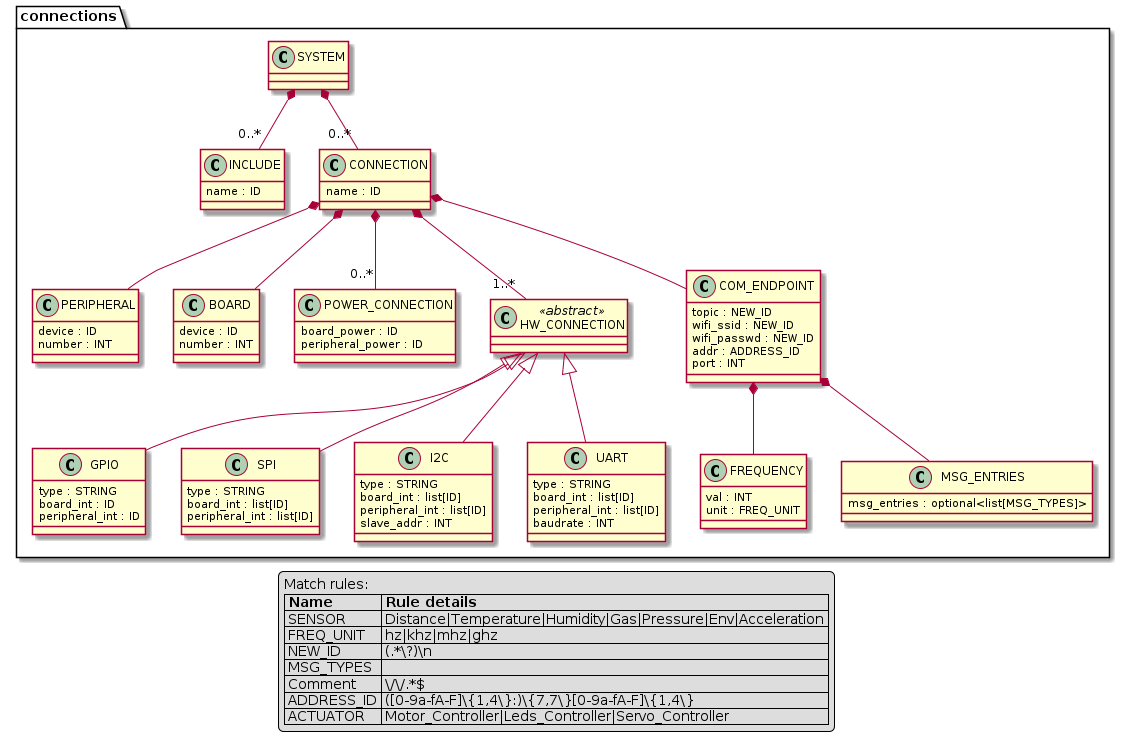
\includegraphics[width=1.0\textwidth]{./images/chapter5/metamodel_connections.png}
	\caption{Μετα-μοντέλο συνδέσεων}
	\label{fig:metamodel_connections}
\end{figure}

\subsection{SYSTEM}
\label{subsec:system}

\subsubsection*{Σύνοψη}

\noindent Το στοιχείο αυτό αναπαριστά ένα σύστημα, το οποίο αποτελείται από συνδέσεις μεταξύ συσκευών. Οι συσκευές αυτές μπορεί να είναι είτε μικροελεγκτές είτε περιφερειακά. 

\subsubsection*{Ιδιότητες και Συσχετίσεις}

\begin{table}[H]
	\begin{center}
		\caption{Συσχετίσεις του \textit{SYSTEM}.}
		\label{tab:system}
		\begin{tabular}{ | c | c | c| m{5.5cm} | }
			\hline
			\rowcolor{Gray}
			Όνομα & Τύπος & Πολλαπλότητα & Περιγραφή \\
			\hline
			INCLUDE & Composition-Σύνθεση & 0..* &  Τα ονόματα των συσκευών που απαρτίζουν το σύστημα \\
			\hline
			CONNECTION & Composition-Σύνθεση & 0..* &  Οι συνδέσεις μεταξύ των συσκευών \\
			\hline
		\end{tabular}
	\end{center}
\end{table}

\noindent Δεν περιλαμβάνει περαιτέρω ιδιότητες.

\subsubsection*{Περιορισμοί}

\noindent Δεν υπάρχουν περιορισμοί.

\subsection{INCLUDE}
\label{subsec:include}

\subsubsection*{Σύνοψη}

\noindent Το στοιχείο αυτό είναι το όνομα μιας συσκευής η οποία είναι μέρος του συστήματος, ώστε να ξέρουμε την ύπαρξή της.

\subsubsection*{Ιδιότητες και Συσχετίσεις}

\begin{table}[H]
	\begin{center}
		\caption{Ιδιότητες του \textit{INCLUDE}.}
		\label{tab:include}
		\begin{tabular}{ | c | c | c| m{5.5cm} | }
			\hline
			\rowcolor{Gray}
			Όνομα & Τύπος & Πολλαπλότητα & Περιγραφή \\
			\hline
			name & ID & 1..1 &  Το όνομα της συσκευής \\
			\hline
		\end{tabular}
	\end{center}
\end{table}

\noindent Δεν περιλαμβάνει περαιτέρω συσχετίσεις.

\subsubsection*{Περιορισμοί}

\noindent Το ID πρέπει να είναι το όνομα συσκευής για την οποία υπάρχει configuration file (.hwd), και άρα να υποστηρίζεται από την παρούσα εργασία.

\subsection{CONNECTION}
\label{subsec:connection}

\subsubsection*{Σύνοψη}

\noindent Το στοιχείο αυτό αναπαριστά τη σύνδεση ενός μικροελεγκτή με ένα περιφερειακό.

\subsubsection*{Ιδιότητες και Συσχετίσεις}

\begin{table}[H]
	\begin{center}
		\caption{Ιδιότητες του \textit{CONNECTION}.}
		\label{tab:connection1}
		\begin{tabular}{ | c | c | c| m{5.5cm} | }
			\hline
			\rowcolor{Gray}
			Όνομα & Τύπος & Πολλαπλότητα & Περιγραφή \\
			\hline
			name & ID & 1..1 &  Το όνομα που θα δοθεί στη σύνδεση \\
			\hline
		\end{tabular}
	\end{center}
\end{table}

\begin{table}[H]
	\begin{center}
		\caption{Συσχετίσεις του \textit{CONNECTION}.}
		\label{tab:connection2}
		\begin{tabular}{ | c | c | c| m{5.5cm} | }
			\hline
			\rowcolor{Gray}
			Όνομα & Τύπος & Πολλαπλότητα & Περιγραφή \\
			\hline
			PERIPHERAL & Composition-Σύνθεση & 1..1 &  Το περιφερειακό της συγκεκριμένης σύνδεσης \\
			\hline
			BOARD & Composition-Σύνθεση & 1..1 &  Ο μικροελεγκτής της συγκεκριμένης σύνδεσης \\
			\hline
			\scriptsize{POWER\_CONNECTION} & Composition-Σύνθεση & 0..* &  Οι ακροδέκτες που χρησιμοποιούνται για την τροφοδοσία \\
			\hline
			\footnotesize{HW\_CONNECTION} & Composition-Σύνθεση & 1..* &  Οι ακροδέκτες που χρησιμοποιούνται για τη σύνδεση μεταξύ των διεπαφών υλικού \\
			\hline
			\small{COM\_ENDPOINT} & Composition-Σύνθεση & 0..1 &  Τα χαρακτηριστικά σύνδεσης σε κάποιον broker \\
			\hline
		\end{tabular}
	\end{center}
\end{table}

\subsubsection*{Περιορισμοί}

\noindent Δεν υπάρχουν περιορισμοί.

\subsection{PERIPHERAL}
\label{subsec:peripheral_con}

\subsubsection*{Σύνοψη}

\noindent Το στοιχείο αυτό περιγράφει το περιφερειακό που χρησιμοποιείται σε μία σύνδεση.

\subsubsection*{Ιδιότητες και Συσχετίσεις}

\begin{table}[H]
	\begin{center}
		\caption{Ιδιότητες του \textit{PERIPHERAL}.}
		\label{tab:peripheral_con}
		\begin{tabular}{ | c | c | c| m{5.5cm} | }
			\hline
			\rowcolor{Gray}
			Όνομα & Τύπος & Πολλαπλότητα & Περιγραφή \\
			\hline
			device & ID & 1..1 & Το όνομα του περιφερειακού \\
			\hline
		    number & INT & 0..1 & Ο αριθμός του περιφερειακού σε περίπτωση που χρησιμοποιείται το ίδιο μοντέλο πολλαπλές φορές στο συγκεκριμένο σύστημα \\
			\hline
		\end{tabular}
	\end{center}
\end{table}

\noindent Δεν περιλαμβάνει περαιτέρω συσχετίσεις.

\subsubsection*{Περιορισμοί}

\noindent Δεν υπάρχουν περιορισμοί.

\subsection{BOARD}
\label{subsec:board_con}

\subsubsection*{Σύνοψη}

\noindent Το στοιχείο αυτό περιγράφει τον μικροελεγκτή που χρησιμοποιείται σε μία σύνδεση.

\subsubsection*{Ιδιότητες και Συσχετίσεις}

\begin{table}[H]
	\begin{center}
		\caption{Ιδιότητες του \textit{BOARD}.}
		\label{tab:board_con}
		\begin{tabular}{ | c | c | c| m{5.5cm} | }
			\hline
			\rowcolor{Gray}
			Όνομα & Τύπος & Πολλαπλότητα & Περιγραφή \\
			\hline
			device & ID & 1..1 & Το όνομα του μικροελεγκτή \\
			\hline
			number & INT & 0..1 & Ο αριθμός του μικροελεγκτή σε περίπτωση που χρησιμοποιείται το ίδιο μοντέλο πολλαπλές φορές στο συγκεκριμένο σύστημα \\
			\hline
		\end{tabular}
	\end{center}
\end{table}

\noindent Δεν περιλαμβάνει περαιτέρω συσχετίσεις.

\subsubsection*{Περιορισμοί}

\noindent Δεν υπάρχουν περιορισμοί.

\subsection{POWER\_CONNECTION}
\label{subsec:power_connection}

\subsubsection*{Σύνοψη}

\noindent Το στοιχείο αυτό περιγράφει τη σύνδεση (ακροδέκτες) τροφοδοσίας των περιφερειακών από τους μικροελεγκτές.

\subsubsection*{Ιδιότητες και Συσχετίσεις}

\begin{table}[H]
	\begin{center}
		\caption{Ιδιότητες του \textit{POWER\_CONNECTION}.}
		\label{tab:power_connection}
		\begin{tabular}{ | c | c | c| m{5.5cm} | }
			\hline
			\rowcolor{Gray}
			Όνομα & Τύπος & Πολλαπλότητα & Περιγραφή \\
			\hline
			board\_power & ID & 1..1 & Ο ακροδέκτης τροφοδοσίας του μικροελεγκτή \\
			\hline
			peripheral\_power & ID & 1..1 & Ο ακροδέκτης τροφοδοσίας του περιφερειακού \\
			\hline
		\end{tabular}
	\end{center}
\end{table}

\noindent Δεν περιλαμβάνει περαιτέρω συσχετίσεις.

\subsubsection*{Περιορισμοί}

\noindent Δεν υπάρχουν περιορισμοί.

\subsection{COM\_ENDPOINT}
\label{subsec:com_endpoint}

\subsubsection*{Σύνοψη}

\noindent Το στοιχείο αυτό περιγράφει τα στοιχεία της σύνδεσης μιας συσκευής σε έναν broker, καθώς και το topic στο οποίο κατά τη λειτουργία της θα κάνει είτε subscribe είτε publish.

\subsubsection*{Ιδιότητες και Συσχετίσεις}

\begin{table}[H]
	\begin{center}
		\caption{Ιδιότητες του \textit{COM\_ENDPOINT}.}
		\label{tab:com_endpoint1}
		\begin{tabular}{ | c | c | c| m{5.5cm} | }
			\hline
			\rowcolor{Gray}
			Όνομα & Τύπος & Πολλαπλότητα & Περιγραφή \\
			\hline
			topic & NEW\_ID & 1..1 & Το όνομα του topic στο οποίο θα στο οποίο θα γίνει publish ή subscribe (ανάλογα αν χρησιμοποιείται αισθητήρας ή ενεργοποιητής αντίστοιχα) \\
			\hline
			wifi\_ssid & NEW\_ID & 1..1 & Το όνομα του wifi δικτύου στο οποίο θα συνδεθεί ο μικροελεγκτής \\
			\hline
			wifi\_password & NEW\_ID & 1..1 & Ο κωδικός του wifi δικτύου στο οποίο θα συνδεθεί ο μικροελεγκτής \\
			\hline
			addr & ADDRESS\_ID & 1..1 & Η IPv6 διεύθυνση του broker με τον οποίο θα επικοινωνήσει ο μικροελεγκτής \\
			\hline
			port & INT & 1..1 & Η πύλη σύνδεσης του broker \\
			\hline
		\end{tabular}
	\end{center}
\end{table}

\begin{table}[H]
	\begin{center}
		\caption{Συσχετίσεις του \textit{COM\_ENDPOINT}.}
		\label{tab:com_endpoint2}
		\begin{tabular}{ | c | c | c| m{5.5cm} | }
			\hline
			\rowcolor{Gray}
			Όνομα & Τύπος & Πολλαπλότητα & Περιγραφή \\
			\hline
			MSG\_ENTRIES & Composition-Σύνθεση & 1..1 &  Τα είδη μηνυμάτων που θα διαμοιραστούν κατά τη συγκεκριμένη σύνδεση \\
			\hline
			FREQUENCY & Composition-Σύνθεση & 0..1 &  Η συχνότητα με την οποία θα γίνονται publish τα μηνύματα στον broker \\
			\hline
		\end{tabular}
	\end{center}
\end{table}

\subsubsection*{Περιορισμοί}

\noindent Τα topic, wifi\_ssid και wifi\_password μπορούν να πάρουν τιμές σαν ID, με επιπλέον επιλογή να περιλαμβάνουν και παύλες. Αυτό επιτυγχάνεται σύμφωνα με το NEW\_ID που είναι μια \textit{κανονική έκφραση} (\textit{regex}).

\noindent Το addr μπορεί να πάρει τιμές σαν μια διεύθυνση \textit{IPv6} (\textit{Internet Protocol version 6}). Αυτό επιτυγχάνεται σύμφωνα με το ADDRESS\_ID που είναι μια \textit{κανονική έκφραση} (\textit{regex}).

\subsection{MSG\_ENTRIES}
\label{subsec:msg_entries}

\subsubsection*{Σύνοψη}

\noindent Το στοιχείο αυτό περιγράφει τα είδη μηνυμάτων που θα διαμοιραστούν σε μια συγκεκριμένη σύνδεση.

\subsubsection*{Ιδιότητες και Συσχετίσεις}

\begin{table}[H]
	\begin{center}
		\caption{Ιδιότητες του \textit{MSG\_ENTRIES}.}
		\label{tab:msg_entries}
		\begin{tabular}{ | c | c | c| m{5.5cm} | }
			\hline
			\rowcolor{Gray}
			Όνομα & Τύπος & Πολλαπλότητα & Περιγραφή \\
			\hline
			msg\_entries & MSG\_TYPES (Enum) & 1..* & Τα είδη μηνυμάτων \\
			\hline
		\end{tabular}
	\end{center}
\end{table}

\noindent Δεν περιλαμβάνει περαιτέρω συσχετίσεις.

\subsubsection*{Περιορισμοί}

\noindent Επιλογές των ειδών μηνυμάτων που μπορούν να δηλωθούν:

\begin{itemize}
	\item Distance
	\item Temperature
	\item Humidity
	\item Gas
	\item Pressure
	\item Env
	\item Acceleration
	\item Motor\_Controller
	\item Leds\_Controller
	\item Servo\_Controller
\end{itemize}

\subsection{HW\_CONNECTION}
\label{subsec:hw_connection}

\subsubsection*{Σύνοψη}

\noindent Το στοιχείο αυτό είναα η abstract κλάση για την περιγραφή των συνδέσεων των διεπαφών υλικών των συσκευών.

\subsubsection*{Ιδιότητες και Συσχετίσεις}

\noindent Δεν περιλαμβάνει περαιτέρω ιδιότητες και συσχετίσεις.

\subsubsection*{Περιορισμοί}

\noindent Δεν υπάρχουν περιορισμοί.

\subsection{GPIO}
\label{subsec:gpio_con}

\subsubsection*{Σύνοψη}

\noindent Το στοιχείο αυτό περιγράφει τη σύνδεση δύο GPIO διεπαφών.

\subsubsection*{Ιδιότητες και Συσχετίσεις}

\begin{table}[H]
	\begin{center}
		\caption{Ιδιότητες του \textit{GPIO}.}
		\label{tab:gpio_con1}
		\begin{tabular}{ | c | c | c| m{5.5cm} | }
			\hline
			\rowcolor{Gray}
			Όνομα & Τύπος & Πολλαπλότητα & Περιγραφή \\
			\hline
			type & STRING & 1..1 & Το είδος διεπαφής (στην προκειμένη περίπτωση gpio) \\
			\hline
			board\_int & ID & 1..1 & Η διεπαφή του μικροελεγκτή \\
			\hline
			peripheral\_int & ID & 1..1 & Η διεπαφή του περιφερειακού \\
			\hline
		\end{tabular}
	\end{center}
\end{table}

\begin{table}[H]
	\begin{center}
		\caption{Συσχετίσεις του \textit{GPIO}.}
		\label{tab:gpio_con2}
		\begin{tabular}{ | c | c | c| m{5.5cm} | }
			\hline
			\rowcolor{Gray}
			Όνομα & Τύπος & Πολλαπλότητα & Περιγραφή \\
			\hline
			\footnotesize{HW\_CONNECTION} & SuperType-Επέκταση & - &  Το στοιχείο GPIO επεκτείνει το στοιχείο HW\_CONNECTION \\
			\hline
		\end{tabular}
	\end{center}
\end{table}

\subsubsection*{Περιορισμοί}

\noindent To type θα πρέπει να έχει την τιμή "gpio", αλλιώς θα εμφανιστεί σφάλμα.

\subsection{I2C}
\label{subsec:i2c_con}

\subsubsection*{Σύνοψη}

\noindent Το στοιχείο αυτό περιγράφει τη σύνδεση μέσω πρωτοκόλλου I2C.

\subsubsection*{Ιδιότητες και Συσχετίσεις}

\begin{table}[H]
	\begin{center}
		\caption{Ιδιότητες του \textit{I2C}.}
		\label{tab:i2c_con1}
		\begin{tabular}{ | c | c | c| m{5.5cm} | }
			\hline
			\rowcolor{Gray}
			Όνομα & Τύπος & Πολλαπλότητα & Περιγραφή \\
			\hline
			type & STRING & 1..1 & Το είδος διεπαφής (στην προκειμένη περίπτωση i2c) \\
			\hline
			board\_int & list[ID] & 1..1 & Οι διεπαφές του μικροελεγκτή \\
			\hline
			peripheral\_int & list[ID] & 1..1 & Οι διεπαφές του περιφερειακού \\
			\hline
			slave\_addr & ID & 1..1 & Η διεύθυνση της διεπαφής που λειτουργεί ως slave \\
			\hline
		\end{tabular}
	\end{center}
\end{table}

\begin{table}[H]
	\begin{center}
		\caption{Συσχετίσεις του \textit{I2C}.}
		\label{tab:i2c_con2}
		\begin{tabular}{ | c | c | c| m{5.5cm} | }
			\hline
			\rowcolor{Gray}
			Όνομα & Τύπος & Πολλαπλότητα & Περιγραφή \\
			\hline
			\footnotesize{HW\_CONNECTION} & SuperType-Επέκταση & - &  Το στοιχείο I2C επεκτείνει το στοιχείο HW\_CONNECTION \\
			\hline
		\end{tabular}
	\end{center}
\end{table}

\subsubsection*{Περιορισμοί}

\noindent To type θα πρέπει να έχει την τιμή "i2c", αλλιώς θα εμφανιστεί σφάλμα.

\subsection{SPI}
\label{subsec:spi_con}

\subsubsection*{Σύνοψη}

\noindent Το στοιχείο αυτό περιγράφει τη σύνδεση μέσω πρωτοκόλλου SPI.

\subsubsection*{Ιδιότητες και Συσχετίσεις}

\begin{table}[H]
	\begin{center}
		\caption{Ιδιότητες του \textit{SPI}.}
		\label{tab:spi_con1}
		\begin{tabular}{ | c | c | c| m{5.5cm} | }
			\hline
			\rowcolor{Gray}
			Όνομα & Τύπος & Πολλαπλότητα & Περιγραφή \\
			\hline
			type & STRING & 1..1 & Το είδος διεπαφής (στην προκειμένη περίπτωση spi) \\
			\hline
			board\_int & list[ID] & 1..1 & Οι διεπαφές του μικροελεγκτή \\
			\hline
			peripheral\_int & list[ID] & 1..1 & Οι διεπαφές του περιφερειακού \\
			\hline
		\end{tabular}
	\end{center}
\end{table}

\begin{table}[H]
	\begin{center}
		\caption{Συσχετίσεις του \textit{SPI}.}
		\label{tab:spi_con2}
		\begin{tabular}{ | c | c | c| m{5.5cm} | }
			\hline
			\rowcolor{Gray}
			Όνομα & Τύπος & Πολλαπλότητα & Περιγραφή \\
			\hline
			\footnotesize{HW\_CONNECTION} & SuperType-Επέκταση & - &  Το στοιχείο SPI επεκτείνει το στοιχείο HW\_CONNECTION \\
			\hline
		\end{tabular}
	\end{center}
\end{table}

\subsubsection*{Περιορισμοί}

\noindent To type θα πρέπει να έχει την τιμή "spi", αλλιώς θα εμφανιστεί σφάλμα.

\subsection{UART}
\label{subsec:uart_con}

\subsubsection*{Σύνοψη}

\noindent Το στοιχείο αυτό περιγράφει τη σύνδεση μέσω πρωτοκόλλου UART.

\subsubsection*{Ιδιότητες και Συσχετίσεις}

\begin{table}[H]
	\begin{center}
		\caption{Ιδιότητες του \textit{UART}.}
		\label{tab:uart_con1}
		\begin{tabular}{ | c | c | c| m{5.5cm} | }
			\hline
			\rowcolor{Gray}
			Όνομα & Τύπος & Πολλαπλότητα & Περιγραφή \\
			\hline
			type & STRING & 1..1 & Το είδος διεπαφής (στην προκειμένη περίπτωση uart) \\
			\hline
			board\_int & list[ID] & 1..1 & Οι διεπαφές του μικροελεγκτή \\
			\hline
			peripheral\_int & list[ID] & 1..1 & Οι διεπαφές του περιφερειακού \\
			\hline
			baudrate & ID & 1..1 & Το baudrate που χρησιμοποιείται \\
			\hline
		\end{tabular}
	\end{center}
\end{table}

\begin{table}[H]
	\begin{center}
		\caption{Συσχετίσεις του \textit{UART}.}
		\label{tab:uart_con2}
		\begin{tabular}{ | c | c | c| m{5.5cm} | }
			\hline
			\rowcolor{Gray}
			Όνομα & Τύπος & Πολλαπλότητα & Περιγραφή \\
			\hline
			\footnotesize{HW\_CONNECTION} & SuperType-Επέκταση & - &  Το στοιχείο UART επεκτείνει το στοιχείο HW\_CONNECTION \\
			\hline
		\end{tabular}
	\end{center}
\end{table}

\subsubsection*{Περιορισμοί}

\noindent To type θα πρέπει να έχει την τιμή "uart", αλλιώς θα εμφανιστεί σφάλμα.

\subsection{FREQUENCY}
\label{subsec:frequency}

\subsubsection*{Σύνοψη}

\noindent Το στοιχείο αυτό περιγράφει τη συχνότητα με την οποία θα γίνονται publish τα μηνύματα στον broker.

\subsubsection*{Ιδιότητες και Συσχετίσεις}

\begin{table}[H]
	\begin{center}
		\caption{Ιδιότητες του \textit{FREQUENCY}.}
		\label{tab:frequency}
		\begin{tabular}{ | c | c | c| m{5.5cm} | }
			\hline
			\rowcolor{Gray}
			Όνομα & Τύπος & Πολλαπλότητα & Περιγραφή \\
			\hline
			val & INT & 1..1 & Η τιμή της συχνότητας \\
			\hline
			val & FREQ\_UNIT & 1..1 & Η μονάδα μέτρησης της συχνότητας \\
			\hline
		\end{tabular}
	\end{center}
\end{table}

\noindent Δεν περιλαμβάνει περαιτέρω συσχετίσεις.

\subsubsection*{Περιορισμοί}

\noindent Επιλογές των υποστηριζόμενων μονάδων μέτρησης για το max\_freq:

\begin{itemize}
	\item hz
	\item khz
	\item ghz
	\item mhz
\end{itemize}
\section{Γραμματική των DSL}
\label{sec:dsl}

Τα μοντέλα που απαρτίζουν την παρούσα εργασία, υπακούουν στους κανόνες που θέτουν τα δύο μετα-μοντέλα που αναλύθηκαν στo \autoref{sec:metamodel_device} και στο \autoref{sec:metamodel_connections}. Για τη δημιουργία τους, αναπτύχθηκαν δύο γλώσσες κειμένου μέσω των οποίων ορίζονται και περιγράφονται οι συσκευές και οι μεταξύ τους συνδέσεις.

Οι γλώσσες αυτές σχεδιάστηκαν με το εργαλείο textX και σε αυτήν την ενότητα περιγράφεται αναλυτικά το συντακτικό τους.

\subsection{Γενικό Συντακτικό}
\label{subsec:syntax}
Και στις δύο γλώσσες που αναπτύχθηκαν, υπάρχουν κάποιοι κοινοί κανόνες συγγραφής.

Αρχικά, κάθε ιδιότητα των μοντέλων δηλώνεται γράφοντας το όνομά της, στη συνέχεια τον χαρακτήρα ":" και τέλος την τιμή της. Για παράδειγμα:

\begin{lstlisting}[title={Παράδειγμα ανάθεσης τιμής σε ιδιότητα}]
	name: value
\end{lstlisting}

Δεύτερος γενικός κανόνας είναι αυτός του τρόπου συγγραφής λίστας. Στην περίπτωση δηλαδή, όπου η τιμή της ιδιότητας είναι μια λίστα από τιμές. Τότε, για κάθε στοιχείο της λίστας γράφουμε αρχικά τον χαρακτήρα "-" και στη συνέχεια τον τύπο του. Για παράδειγμα, τα pins μιας συσκευής μπορεί να είναι power, io\_pin, input\_pin ή output\_pin. Οπότε κάποια από τα pins ενός αισθητήρα θα μπορούσαν να είναι τα εξής.

\begin{lstlisting}[title={Παράδειγμα ορισμού pins αισθητήρα}]
	pins:
		- power:
			name: vcc
			number: 1
			type: 5v
		- input_pin:
			name: data_in
			number: 3
		- output_pin:
			name: data_out
			number: 4
\end{lstlisting}

\subsection{Συντακτικό Συσκευής}
\label{subsec:syntax_device}

Μια συσκευή μπορεί να είναι είτε μικροελεγκτής είτε περιφερειακό (αισθητήρας/ενεργοποιητής). Στην αρχή του αρχείο το πρώτο που δηλώνουμε είναι αυτό, γράφοντας "Board:" για τους μικροελεγκτές και "Peripheral:" για τα περιφερειακά. Τα περισσότερα χαρακτηριστικά είναι κοινά και για τα δύο, επομένως ότι εξηγηθεί παρακάτω εφαρμόζεται με τον ίδιο τρόπο είτε έχουμε μικροελεγκτή είτε περιφερειακό. Στο τέλος θα αναλυθούν ξεχωριστά τα χαρακτηριστικά που δηλώνονται μόνο για μικροελεγκτή και αυτά που δηλώνονται μόνο για περιφερειακό.

Αξίζει να σημειωθεί πως τα χαρακτηριστικά για την κάθε συσκευή, δεν έχει σημασία με ποια σειρά θα δηλωθούν.

\subsubsection{Βασικές Ιδιότητες}
Κάποιες ιδιότητες είναι αρκετά εύκολο να συγγραφούν, καθώς αποτελούν μια απλή ανάθεση τιμής. Ο τρόπος συγγραφής τους είναι ο ακόλουθος:

\begin{lstlisting}
	name: value
	riot_name: value
	vcc: value
	operating_voltage: value
\end{lstlisting}

Το name είναι το όνομα που δίνουμε στη συσκευή και δέχεται ως τιμή αλφαριθμητικό. Το riot\_name είναι το όνομα της συσκευής όπως αναγνωρίζεται από το RIOT, και δέχεται ως τιμή αλφαριθμητικό με επιπλέον επιλογή να περιλαμβάνει και παύλες. Το vcc και το operating\_voltage είναι η τάση τροφοδοσίας και η τάση λειτουργίας της συσκευής αντίστοιχα, και παίρνουν ως τιμή αριθμό κινητής υποδιαστολής.

\subsubsection{Pins}

Για τα pins της εκάστοτε συσκευής, δηλώνουμε το είδος του pin, και ανάλογα το είδος μπορεί να έχει συγκεκριμένα χαρακτηριστικά. Ο γενικός τρόπος σύνταξης είναι ο ακόλουθος (όπου μπορούμε να έχουμε πολλά pins και το καθένα να έχει πολλά χαρακτηριστικά):

\begin{lstlisting}
	pins:
		- pin_type:
			attribute: value
\end{lstlisting}

Το είδος pin μπορεί να είναι ένα εκ των "power", "io\_pin", "input\_pin" και "output\_pin". Σε όλες τις περιπτώσεις, όπου name είναι είναι ένα αλφαριθμητικό που δηλώνει το όνομα του ακροδέκτη, και number ένας ακέραιος αριθμός που υποδηλώνει την θέση του ακροδέκτη στη συσκευή. Επίσης, όπου υπάρχει το vmax υποδηλώνει την μέγιστη τιμή τάσης που μπορει να δεχτεί ο ακροδέκτης (η συγκεκριμένη ιδιότητα δεν είναι υποχρεωτική).

\textbf{\underline{power}}

\begin{lstlisting}
	power:
		name: value
		number: value
		type: value
\end{lstlisting}

Όπου type πρέπει να είναι ένα εκ των "gnd", "5v" και "3v3".

\textbf{\underline{input\_pin}}

\begin{lstlisting}
	input_pin:
		name:value
		number: value
		vmax: value
\end{lstlisting}

\textbf{\underline{output\_pin}}

\begin{lstlisting}
	output_pin:
		name:value
		number: value
		vmax: value
\end{lstlisting}

\textbf{\underline{io\_pin}}

\begin{lstlisting}
	io_pin: -> function1, function2, function3
		name:value
		number: value
		vmax: value
\end{lstlisting}

Το io\_pin πέρα από τα name, number και vmax, έχει μια επιπλέον ιδιότητα, η οποία είναι οι λειτουργίες που μπορεί να έχει. Για να τις ορίσουμε, αρχικά γράφουμε τους χαρακτήρες "->" και στη συνέχεια γράφουμε τις λειτουργίες, χωρίζοντάς τες με το χαρακτήρα "," (εφόσον είναι περισσότερες από μία). Οι λειτουργίες που μπορεί να έχει ένας ακροδέκτης είναι οι ακόλουθες:

\begin{itemize}
	\item gpio
	\item sda: SDA σε I2C διεπαφή
	\item scl: SCL σε I2C διεπαφή
	\item mosi: MOSI σε SPI διεπαφή
	\item miso: MISO σε SPI διεπαφή
	\item sck: SCK σε SPI διεπαφή
	\item cs: CS σε SPI διεπαφή
	\item tx: TX σε UART διεπαφή
	\item rx: RX σε UART διεπαφή
	\item pwm
	\item adc
	\item dac
\end{itemize}

Στην περίπτωση των pin τύπου I2C, SPI, UART και PWM ακολουθεί και ο χαρακτήρας "-" ώστε μετά από αυτόν να μπει ένας αριθμός, ο οποίος συμβολίζει τον αριθμό της διεπαφής στην οποία ανήκει το pin.

Ένα παράδειγμα με μερικά από τα pins ενός μικροελεγκτή θα μπορούσε να είναι το ακόλουθο:

\begin{lstlisting}
	pins:
		...
		...
		- power:
			name: gnd_1
			number: 14
			type: gnd
		- io_pin: -> gpio, mosi-1, adc
			name: p_13
			number: 15
		- io_pin: -> gpio, rx-1
			name: p_9
			number: 16
		- io_pin: -> gpio, tx-1
			name: p_10
			number: 17
		- io_pin: -> gpio
			name: p_11
			number: 18
		- power:
			name: power_5v
			number: 19
			type: 5v
		...
		...
\end{lstlisting}

\subsubsection{Επιπλέον χαρακτηριστικά ενός Board}

\textbf{\underline{Memory}}

\begin{lstlisting}
	memory:
		ram: value unit
		rom: value unit
		flash: value unit
\end{lstlisting}

Όπου value είναι ακέραιος αριθμός που δηλώνει το μέγεθος της μνήμης και unit μπορεί να είναι ένα εκ των "b", "mb", "kb" και "gb". Δεν χρειάζεται να περιλαμβάνονται και τα τρία είδη μνήμης (ram, rom, flash), αλλά τουλάχιστον ένα από αυτά.

\textbf{\underline{Cpu}}

\begin{lstlisting}
	cpu:
		cpu_family: value
		max_freq: value unit
		fpu: value
\end{lstlisting}

Όπου cpu\_family ένα εκ των "ESP32" και "ESP8266". Το max\_freq παίρνει ως τιμή έναν αριθμό, και το unit παίρνει για τιμή ένα εκ των "hz", "ghz" και "mhz". Τέλος το fpu είναι είναι τύπου boolean.
2990
\textbf{\underline{Network}}

\begin{lstlisting}
	network:
		- network_type:
			attribute: value
\end{lstlisting}

Όπου network\_type είναι ένα εκ των "wifi" και "ethernet". Όπως βλέπουμε και παρακάτω, και στις δύο περιπτώσεις υπάρχει το όνομα (name) του δικτύου το οποίο δέχεται ως τιμή ένα αλφαριθμητικό. Στην περίπτωση του wifi έχουμε επιπλεόν την επιλογή freq η οποία δέχεται ως value έναν αριθμό, και ως unit ένα εκ των "hz", "mhz" και "ghz". Το network δεν είναι υποχρεωτικό στοιχείο.

- wifi

\begin{lstlisting}
	wifi:
		name: value
		freq: value unit
\end{lstlisting}

- ethernet

\begin{lstlisting}
	ethernet:
		name: value
\end{lstlisting}

\textbf{\underline{Bluetooth}}

\begin{lstlisting}
	bluetooth:
		version: value
\end{lstlisting}

Η τιμή της έκδοσης (version) είανι ένας αριθμός. Το bluetooth δεν είναι υποχρεωτικό στοιχείο.

\subsubsection{Επιπλέον χαρακτηριστικά ενός Peripheral}

\textbf{\underline{Type}}

\begin{lstlisting}
	type: value
\end{lstlisting}

Το μόνο επιπλέον χαρακτηριστικό που έχει ένα περιφερειακό πέρα από τις βασικές ιδιότητες, είναι ο τύπος, που μπορεί να έχει ως τιμή ένα εκ των "sensor" και "actuator".

\subsection{Συντακτικό Συνδέσεων}
\label{subsec:syntax_connections}

Κάθε μοντέλο βασισμένο στο μετα-μοντέλο συνδέσεων αποτελείται από ένα σύστημα. Το σύστημα αυτό αποτελείται από μία ή περισσότερες συνδέσεις μεταξύ μικροελεγκτών και περιφερειακών. Κάθε μία από τις συσκευές που χρησιμοποιείται στο σύστημα, αρχικά πρέπει να δηλωθεί με την ακόλουθη σύνταξη:

\begin{lstlisting}
	include value
\end{lstlisting}

Όπου value το όνομα της εκάστοτε συσκευής, όπως έχει δοθεί στο configuration file της (αρχείο κατασκευασμένο σύμφωνα με τους κανόνες του συντακτικού που αναλύεται στην \autoref{subsec:syntax_device})).

Στη συνέχεια, για κάθε μία από τις συνδέσεις που υπάρχουν στο σύστημα, γράφεται η λέξη "connection" και ο χαρακτήρας ":" και ακολουθούν οι ιδιότητές της.

\subsubsection{Ιδιότητες}

Αρχικά βλέπουμε τρεις ιδιότητες (name, board, peripheral) οι οποίες έχουν αρκετά απλή σύνταξη, απλής ανάθεσης τιμής.

\begin{lstlisting}
	connection:
		name: value
		board: value (number)
		peripheral: value (number)
\end{lstlisting}

Και οι τρεις ιδιότητες παίρνουν ως value κάποιο αλφαριθμητικό. To board και το peripheral έχουν και την επιλογή (όχι υποχρεωτικό) να έχουν και έναν αναγνωριστικό αριθμό (το number), τοποθετημένο ανάμεσα στους χαρακτήρες "(" και ")". Η δυνατότητα αυτή παρέχεται για την περίπτωση όπου σε πολλαπλές συνδέσεις χρησιμοποιείται συσκευή με το ίδιο όνομα.

\textbf{\underline{power\_connections}}

\begin{lstlisting}
	power_connection:
		- board_pin1 -- peripheral_pin1
		- board_pin2 -- peripheral_pin2
		...
		...
\end{lstlisting}

Η συνδέσεις τροφοδοσίας συντάσσονται ως μια λίστα από αντιστοιχίσεις των pins του μικροελεγκτή, με αυτά του περιφερειακού. Άρα για κάθε σύνδεση pin, αρχικά αναγράφεται το όνομα του pin του μικροελεγκτή, και στη συνέχεια το όνομα του pin του περιφερειακού. Τα δύο ονόματα διαχωρίζονται από τους χαρακτήρες "--". Κάθε στοιχείο της λίστας ξεκινάει με τον χαρακτήρα "-".

\textbf{\underline{hw\_connections}}

Η συνδέσεις διεπαφών υλικού, έχουν διαφορετικό τρόπο σύνταξης ανάλογα με τον τύπο της σύνδεσης. Οι τύποι σύνδεσης που υποστηρίζονται είναι οι ακόλουθοι:

\begin{itemize}
	\item gpio
	\item i2c
	\item spi
	\item uart
\end{itemize}	

Ωστόσο, σε όλες τις περιπτώσεις η σύνταξη ξεκινάει με τον χαρακτήρα "-", τον τύπο σύνδεσης και τέλος τον χαρακτήρα ":", όπως φαίνεται παρακάτω (όπου type ο τύπος):

\begin{lstlisting}
	- type:
\end{lstlisting}

$\rightarrow$ \underline{\textit{gpio}}

\begin{lstlisting}
	hw_connections:
		...
		...
		- gpio: board_pin1 -- peripheral_pin1
		- gpio: board_pin2 -- peripheral_pin2
		...
		...
\end{lstlisting}

Οι συνδέσεις gpio συντάσσονται ακριβώς όπως οι συνδέσεις τροφοδοσίας, με τη μόνη προσθήκη του "gpio:" το οποίο είναι ο τύπος σύνδεσης όπως αναφέρθηκε προηγουμένως.

$\rightarrow$ \underline{\textit{i2c}}

\begin{lstlisting}
	hw_connections:
		...
		...
		- i2c: 
			sda: board_pin -- peripheral_pin
			scl: board_pin -- peripheral_pin
			slave_address: value
		...
		...
\end{lstlisting}

Οι συνδέσεις i2c συντάσσονται αρχικά με τον τύπο της σύνδεσης ("- i2c:) και στη συνέχεια μια λίστα με τα στοιχεία της σύνδεσεις αυτής. Τα sda και scl συντάσσονται όπως και το gpio, ενώ το slave\_address παίρνει τιμή έναν δεκαεξαδικό αριθμό της μορφής "0x00" (πρώτα οι χαρακτήρες "0x" και στη συνέχεια ο δεκαεξαδικός).

$\rightarrow$ \underline{\textit{spi}}

\begin{lstlisting}
	hw_connections:
		...
		...
		- spi: 
			mosi: board_pin -- peripheral_pin
			miso: board_pin -- peripheral_pin
			sck: board_pin -- peripheral_pin
			cs: board_pin -- peripheral_pin
		...
		...
\end{lstlisting}

Οι συνδέσεις spi συντάσσονται αρχικά με τον τύπο της σύδεσης ("- spi:") και στη συνέχεια όπως και οι συνδέσεις i2c, με τη διαφορά ότι δεν υπάρχει slave\_address, και τα είδη των pin αντί για sda και scl είναι mosi, miso, sck και cs.

$\rightarrow$ \underline{\textit{uart}}

\begin{lstlisting}
	hw_connections:
		...
		...
		- uart: 
			tx: board_pin -- peripheral_pin
			rx: board_pin -- peripheral_pin
			baudrate: value
		...
		...
\end{lstlisting}

Οι συνδέσεις uart συντάσσονται αρχικά με τον τύπο της σύδεσης ("- uart:") και στη συνέχεια όπως και οι συνδέσεις i2c, με τη διαφορά ότι αντί για slave\_address υπάρχει το στοιχείο baudrate, που παίρνει ως τιμή κάποιον ακέραιο αριθμό, και τα είδη των pin αντί για sda και scl είναι tx και rx.

\textbf{\underline{communication\_endpoint}}

\begin{lstlisting}
	communication_endpoint:
		topic: value
		wifi_ssid: value
		wifi_passwd: value
		address: value
		port: value
		msg: value
		frequency: value unit
\end{lstlisting}

Τελευταία ιδιότητας μιας σύνδεσης είναι τα χαρακτηριστικά για τη σύνδεση σε κάποιον broker. Τα topic, wifi\_ssid και wifi\_password παίρνουν ως τιμή κάποια αλληλουχία γραμμάτων, αριθμών και συμβόλων χωρίς κενά. Το στοιχείο address παίρνει ως τιμή μια διεύθυνση τύπου IPv6 καιτο port κάποιον ακέραιο αριθμό. Το frequency (το οποίο δεν είναι υποχρεωτικό) παίρνει ως τιμή κάποιον ακέραιο και ως unit ένα εκ των "hz", "khz", "mhz" και "ghz".

Τέλος το msg είναι το είδος του μηνύματος που θα γίνει publish ή θα ληφθεί από κάποιον subscriber και μπορεί να είναι ένα εκ των "Distance", "Temperature", "Humidity", "Gas", "Pressure", "Env", "Acceleration", "Motor\_Controller", "Leds\_Controller", "Servo\_Controller".
\section{Μετασχηματισμός M2M}
\label{sec:transformation}

Αφού δημιουργηθούν τα κατάλληλα αρχεία περιγραφής συσκευών και συνδέσεων, σύμφωνα με τους κανόνες των συντακτικών που αναλύθηκαν στο \autoref{sec:dsl} ξεκινάει η κύρια διαδικασία της παρούσας εργασίας.

Πρώτο βήμα, είναι η δημιουργία μοντέλων για κάθε μια από της συσκευές που χρησιμοποιούνται στην εκάστοτε υλοποίηση, αλλά και για τις μεταξύ τους συνδέσεις. Πριν όμως γίνει η παραγωγή του κατάλληλου κώδικα, που θα αναλυθεί στην επόμενη ενότητα, δημιουργούνται δύο διαγράμματα για το μοντέλο των συνδέσεων, τα οποία βοηθούν στην οπτικοποίηση και άρα καλύτερη αντίληψη από τον χρήστη για τη συνδεσμολογία και ενδοεπικοινωνία του συστήματός του.

Το πρώτο διάγραμμα είναι η παρουσίαση όλων των χαρακτηριστικών των συνδέσεων με τη μορφή οντοτήτων, ενώ το δεύτερο είναι μια οπτικοποίηση των αντιστοιχίσεων των ακροδεκτών με τους οποίους συνδέονται οι συσκευές μεταξύ τους, αλλά και των topic στα οποία επικοινωνεί η εκάστοτε συσκευή.

Για την παραγωγή των διαγραμμάτων αυτών, γίνεται χρήση του εργαλείου PlantUML. Για την παραγωγή των PlantUML αρχείων (βασισμένα στην DSL που το εργαλείο αυτό υποστηρίζει), γίνεται αρχικά ένας M2M μετασχηματισμός του μοντέλου συνδέσεων στο μοντέλο της DSL του PlantUML. Ο μετασχηματισμός αυτός πραγματοποιείται μέσω δύο \textit{python modules}\footnote{\url{https://docs.python.org/3/tutorial/modules.html}} που δημιουργήθηκαν στα πλαίσια της παρούσας διπλωματικής εργασίας. Ένα παράδειγμα από το κάθε διάγραμμά παρουσιάζεται στο \autoref{appendix:diagrams}.
\section{Παραγωγή κώδικα}
\label{sec:generation}

Σε αυτήν την ενότητα θα εξεταστεί η διαδικασία παραγωγής αρχείων κώδικα από την παρούσα εργασία. Τα αρχεία που παράγονται είναι δύο, ένα αρχείο σε γλώσσα C και ένα αρχείο Makefile, από τα οποία θα παραχθεί ένα εκτελέσιμο για να φορτωθεί σε κάποιον μικροελεγκτή. Τα αρχεία αυτά παράγονται μέσω κάποιων \textit{πρότυπων αρχείων} (\textit{templates}) που δημιουργήθηκαν στα πλαίσια της διπλωματικής. Τα πρότυπα αρχεία παρουσιάζονται στο \autoref{appendix:templates}.

Όπως αναφέρθηκε στο \autoref{sec:transformation} αρχικά παράγονται τα μοντέλα για κάθε μια από της συσκευές που χρησιμοποιούνται στην εκάστοτε υλοποίηση, αλλά και για τις μεταξύ τους συνδέσεις. Η πληροφορία που αντλείται από τα μοντέλα, δίνεται ως παράμετροι στα πρότυπα αρχεία. Με αυτόν τον τρόπο, από τα πρότυπα αρχεία παράγονται τα τελικά αρχεία προς εκτέλεση. Παρακάτω αναλύονται κάποιες βασικές συναρτήσεις και λειτουργίες που υλοποιούνται από τα πρότυπα αρχεία.

\subsection{Αρχείο κώδικα C}
\label{subsec:c_code}

\subsubsection{Επικοινωνία με broker}

\noindent Για την επικοινωνία του μικροελεγκτή με κάποιον broker υλοποιήθηκαν οι παρακάτω συναρτήσεις.

\noindent\begin{minipage}{\textwidth}
\noindent $\bullet$ con( addr , port )

\begin{table}[H]
	\centering
	\begin{tabular}{|c|c|}
		\hline
		\rowcolor{Gray}
		\multicolumn{2}{|c|}{\textbf{Περιγραφή}} \\ 
		\hline
		\multicolumn{2}{|c|}{Σύνδεση στον broker} \\ 
		\hline
		\rowcolor{Gray}
		\multicolumn{2}{|c|}{\textbf{Ορίσματα}}  \\
		\hline
		\rowcolor{Gray} 
		Όρισμα & Επεξήγηση \\
		\hline
		addr & IPv6 διεύθυνση του broker \\ 
		\hline
		port & Πύλη επικοινωνίας MQTT-SN \\
		\hline
	\end{tabular}
	\label{tab:con}
\end{table}
\end{minipage}

\noindent\begin{minipage}{\textwidth}
\noindent $\bullet$ discon( )

\begin{table}[H]
	\centering
	\begin{tabular}{|c|c|}
		\hline
		\rowcolor{Gray}
		\multicolumn{2}{|c|}{\textbf{Περιγραφή}} \\ 
		\hline
		\multicolumn{2}{|c|}{Αποσύνδεση από τον broker} \\ 
		\hline
		\rowcolor{Gray}
		\multicolumn{2}{|c|}{\textbf{Ορίσματα}}  \\
		\hline
		\multicolumn{2}{|c|}{\textbf{-}}  \\
		\hline
	\end{tabular}
	\label{tab:discon}
\end{table}
\end{minipage}

\noindent\begin{minipage}{\textwidth}
	\noindent $\bullet$ pub(topic, data, qos)
	
	\begin{table}[H]
		\centering
		\begin{tabular}{|c|c|}
			\hline
			\rowcolor{Gray}
			\multicolumn{2}{|c|}{\textbf{Περιγραφή}} \\ 
			\hline
			\multicolumn{2}{|c|}{Publish κάποιου μηνύματος σε συγκεκριμένο topic} \\ 
			\hline
			\rowcolor{Gray}
			\multicolumn{2}{|c|}{\textbf{Ορίσματα}}  \\
			\hline
			\rowcolor{Gray} 
			Όρισμα & Επεξήγηση \\
			\hline
			topic & Topic στο οποίο θα γίνει το publish \\ 
			\hline
			data & Το μήνυμα που πρόκειται να γίνει publish \\
			\hline
			qos & Ποιότητα υπηρεσιών (Quality of Service) \\
			\hline
		\end{tabular}
		\label{tab:pub}
	\end{table}
\end{minipage}

\noindent\begin{minipage}{\textwidth}
	\noindent $\bullet$ sub(topic, qos, func)
	
	\begin{table}[H]
		\centering
		\begin{tabular}{|c|M{13cm}|}
			\hline
			\rowcolor{Gray}
			\multicolumn{2}{|c|}{\textbf{Περιγραφή}} \\ 
			\hline
			\multicolumn{2}{|c|}{Publish κάποιου μηνύματος σε συγκεκριμένο topic} \\ 
			\hline
			\rowcolor{Gray}
			\multicolumn{2}{|c|}{\textbf{Ορίσματα}}  \\
			\hline
			\rowcolor{Gray} 
			Όρισμα & Επεξήγηση \\
			\hline
			topic & Topic στο οποίο θα "ακούει" \\ 
			\hline
			qos & Ποιότητα υπηρεσιών (Quality of Service) \\
			\hline
			func & Η συνάρτηση που θα είναι υπεύθυνη για την εκτέλεση λειτουργιών σε περίπτωση κάποιου publish \\
			\hline
		\end{tabular}
		\label{tab:sub}
	\end{table}
\end{minipage}

\subsubsection{Sensor}

\noindent $\bullet$ send\_<sensor\_name>( )

\noindent Στην περίπτωση που χρησιμοποιείται αισθητήρας, η συνάρτησή αρχικά κάνει εκκίνηση του αισθητήρα, πραγματοποιεί μία μέτρηση, και τέλος την κάνει publish στο αντίστοιχο topic στον broker. Όπου sensor\_name θα εμφανιστεί το όνομα του αισθητήρα.

\subsubsection{Actuator}

\noindent $\bullet$ receive\_<actuator\_name>( )

\noindent Η συνάρτηση αυτή είναι υπεύθυνη ώστε κάθε φορά που γίνεται publish στο αντίστοιχο topic, να καλεί την επόμενη συνάρτηση ( \textit{<actuator\_name>\_on\_pub( )} ) ώστε να εκτελείται η διαδικασία για τους ενεργοποιητές. Όπου actuator\_name θα εμφανιστεί το όνομα του ενεργοποιητή.

\noindent $\bullet$ <actuator\_name>\_on\_pub( )

Στην περίπτωση όπου γίνει κάποιο publish στο αντίστοιχο topic, η συνάρτηση αυτή είναι υπεύθυνη ώστε να αποθηκεύσει το μήνυμα, να κάνει εκκίνηση του ενεργοποιητή και τέλος να δράσει ανάλογα με το είδος του ενεργοποιητή. Όπου actuator\_name θα εμφανιστεί το όνομα του ενεργοποιητή.

\subsection{Αρχείο Makefile}
\label{subsec:makefile}

Το Makefile είναι αρχείο απαραίτητο για να γίνει compile του εκτελέσιμου κώδικα C. Στο RIOT υπάρχουν κάποια υλοποιημένα modules τα οποία μπορούν να χρησιμοποιηθούν στις εφαρμογές που αναπτύσσονται με το λειτουργικό αυτό. Στο Makefile γίνονται τα includes των απαραίτητων modules. Στην παρούσα εργασία χρησιμοποιούνται modules που είναι υπεύθυνα για λειτουργίες δικτύωσης, χρονοδιακοπτών, καθώς και τα modules όλων των περιφερειακών που χρησιμοποιούνται στην εκάστοτε υλοποίηση.

Το όνομα της υλοποίησης, τα ονόματα των περιφερειακών και του μικροελεγκτή καθώς και τα στοιχεία του wifi στο οποίο θα συνδεθεί, δίνονται ως παράμετροι στο πρότυπο αρχείο Makefile.
\section{Υποστηριζόμενες συσκευές}
\label{sec:supported}

Για να υποστηρίζεται κάποια συσκευή από τη διαδικασία, είναι απαραίτητο να έχουν πρώτα συγγραφεί κάποια συγκεκριμένα αρχεία.

Στην περίπτωση κάποιου μικροελεγκτή, χρειάζεται να υπάρχει το αντίστοιχο configuration αρχείο (.hwd) σύμφωνα με το συντακτικό  που αναλύεται στην \autoref{subsec:syntax_device}.

Στην περίπτωση κάποιου περιφερειακού, χρειάζεται να υπάρχει το αντίστοιχο configuration αρχείο (.hwd) σύμφωνα με το συντακτικό  που αναλύεται στην \autoref{subsec:syntax_device}, αλλά και ένα πρότυπο αρχείο κώδικα C, στο οποίο υλοποιούνται κάποιες βασικές λειτουργίες οι οποίες αναλύονται στην \autoref{subsec:c_code}.

Στα πλαίσια της παρούσας διπλωματικής εργασίας, γράφτηκαν πρότυπα αρχεία, και configuration αρχεία (.hwd) για 2 μικροελεγκτές, 3 σένσορες και 1 ενεργοποιητή. Οι συσκευές αυτές είναι οι ακόλουθες:

\begin{itemize}
	\item NODEMCU ESP-32S\footnote{\url{https://docs.ai-thinker.com/_media/esp32/docs/nodemcu-32s_product_specification.pdf}}
	\item WEMOS D1 miniPro\footnote{\url{https://www.wemos.cc/en/latest/d1/d1_mini.html}}
	\item Αισθητήρας αποστασης HC-SR04\footnote{\url{https://www.sparkfun.com/products/15569}}
	\item Αισθητήρας περιβάλλοντος BME680\footnote{\url{https://shop.pimoroni.com/products/bme680-breakout}}
	\item Αισθητήρας περιβάλλοντος MPL3115A2\footnote{\url{https://www.adafruit.com/product/1893}}
	\item Ενεργοποιητής LED NeoPixel Ring\footnote{\url{https://www.adafruit.com/product/1643}}
\end{itemize}
